\documentclass{article}

\usepackage{xcolor}
\usepackage{graphicx}
\graphicspath{ {./figures/} }
\usepackage{amsmath}
\usepackage{amssymb}
\usepackage{amsthm}
\usepackage{float}
\usepackage{placeins}
\usepackage{hyperref}
\usepackage{cleveref}
\usepackage{booktabs}
\usepackage{minted}
\usepackage{csquotes}

\newcommand{\assoc}{\oplus}
\newcommand{\conj}{\wedge}
\newcommand{\disj}{\vee}
\newcommand{\concat}{\ensuremath{\mathbin{+\mkern-10mu+}}}
\newcommand{\compose}{\ensuremath{\mathbin{\circ}}}
\newcommand{\map}{\ensuremath{\mathbin{\ast}}}
\newcommand{\crossop}{\ensuremath{\mathbin{\mathcal{X}}}}
\newcommand{\maxop}{\uparrow}
\newcommand{\minop}{\downarrow}


\begin{document}

\title{DPP Assignment 4}
\author{Cornelius Sevald-Krause \\ \texttt{<lgx292>}}
\date{2022-12-23}
\maketitle

\section*{Task 1}

The source code for the \verb|matrix_inverse| function as well as the
\verb|main| function is shown in~\cref{lst:matrixinv}.

\begin{listing}[t]
    \centering
    \begin{minted}{futhark}
        def matrix_inverse [n] (A: [n][n]f32): [n][n]f32 =
          let AI =
            let I = scatter (replicate (n*n) 0)
                            (map (\i -> i+n*i) (iota n))
                            (replicate n 1)
                          |> unflatten n n
            in map2 (concat_to (2*n)) A I
          let BAinv = gaussian_elimination AI
          let Ainv = BAinv[0:n,n:2*n] :> [n][n]f32
          in Ainv

        entry main [k] [n] (As: [k][n][n]f32) : [k][n][n]f32 =
          map matrix_inverse As
    \end{minted}
    \caption{\texttt{matrix\_inverse} and \texttt{main} function.}
    \label{lst:matrixinv}
\end{listing}

To figure out how many levels of parallelism the program exhibits, we inline the
function calls, starting from \verb|main|, and keep just the \textsc{soac}s:
\begin{Verbatim}[commandchars=\\\{\}]
map matrix_inverse As
├─replicate n 1
├─replicate (n*n) 0
├─map ({\textbackslash}i -> i+n*i) (iota n)
├─scatter ...
├─map2 (concat_to (2*n)) A I
└─loop A for i < i64.min m n do
  ├─map2 value (indices A)
  ├─reduce_comm ...
  ├─map2 (f32.fma f) A[j] A[i]
  └─map2 ({\textbackslash}x y -> ...) irow A[j]
\end{Verbatim}
From this we see that there is an outer level of parallelism in which we
\verb|map| \verb|matrix_inverse| over the list of matrices, and an inner level
of parallelism, which is all of the leaf node \textsc{soac}s. The extra nested
level of the \verb|loop| does not count as \verb|loop|s are sequential.

\vspace{1em}

\noindent
The relevant sections of the internal representation of
\verb|matrix-inversion.fut| is shown in~\cref{lst:matrixinv_internals}.
% First `if`
The first \texttt{if}-statement (l. 129) checks if there is sufficient outer
parallelism at the current level, and if so, sequentializes the map body, which
is the entire \verb|matrix_inverse| function.
% Second `if`
The second \texttt{if}-statement (l. 291) determines whether or not the
remaining code should be preformed at the block-level. The
remaining code being the \verb|matrix_inverse| function.
% Third `if`
The third \texttt{if}-statement (l. 476) again checks if there is sufficient
outer parallelism at the current level, and if so, sequentializes the map body,
which is the \verb|gaussian_elimination| function.
% Fourth if
The second \texttt{if}-statement (l. 604) again determines whether or not the
remaining code should be preformed at the block-level. In this case the
remaining code is the \verb|gaussian_elimination| function.

\begin{listing}[t]
    \begin{Verbatim}[frame=single,commandchars=\\\{\}]
{\footnotesize 129:} if <equiv> suff_outer_par_9568
{\footnotesize 130:} then \{ \ldots
{\footnotesize 289:} \} else \{ \ldots
{\footnotesize 291:}   if <equiv> intra_suff_and_fits_9732
{\footnotesize 292:}   then \{ \ldots
{\footnotesize 445:}   \} else \{ \ldots
{\footnotesize 476:}     if <equiv> suff_outer_par_10671
{\footnotesize 477:}     then \{ \ldots
{\footnotesize 602:}     \} else \{ \ldots
{\footnotesize 604:}       if <equiv> intra_suff_and_fits_10683
{\footnotesize 605:}       then \{ \ldots
{\footnotesize 724:}       \} else \{ \ldots
{\footnotesize 863:}       \}
{\footnotesize 866:}     \}
{\footnotesize 881:}   \}
{\footnotesize 884:} \}
    \end{Verbatim}
    \caption{Relevant sections of \texttt{matrix-inversion.fut} internals.}
    \label{lst:matrixinv_internals}
\end{listing}

The benchmarks of shape \texttt{[k][n][n]} range from $k = 64, \ldots , 1048576$
and $n = 128, \ldots , 1$ and are set up such that $k \cdot n \cdot n =
1048576$. I preformed the benchmarks with no tuning file and with an
auto-generated tuning file and plotted the results, which are shown
in~\cref{fig:matrix_inv_bench}. The benchmarks were done with Futhark version
0.21.4 on the \verb|gpu04-diku-apl| machine. You should be able to run (and
plot) the benchmarks by just running \verb|make| in the \verb|code-handout/|
directory.

The performance of the untuned version is similar to that of the tuned version
for most of the input sizes, but for inputs where $k = 2^{12}$ to $k=2^{16}$ the
tuned version is a good bit faster (speedup of \textapprox 3x). The reason
for this can be found by looking at the result of the auto-tuning:
\begin{Verbatim}
Result of autotuning:
main.suff_intra_par_1=4
main.suff_intra_par_3=4
main.suff_outer_par_0=64
main.suff_outer_par_2=256
\end{Verbatim}
That \verb|suff_intra_par_1| and \verb|suff_intra_par_1| are equal to 4 suggests
that when $n=4$ (in which case $k=2^{16}$) the tuned version will use a
different strategy to the untuned version, which explains the speedup at $k =
2^{16}$.

\begin{figure}[t]
    \centering
    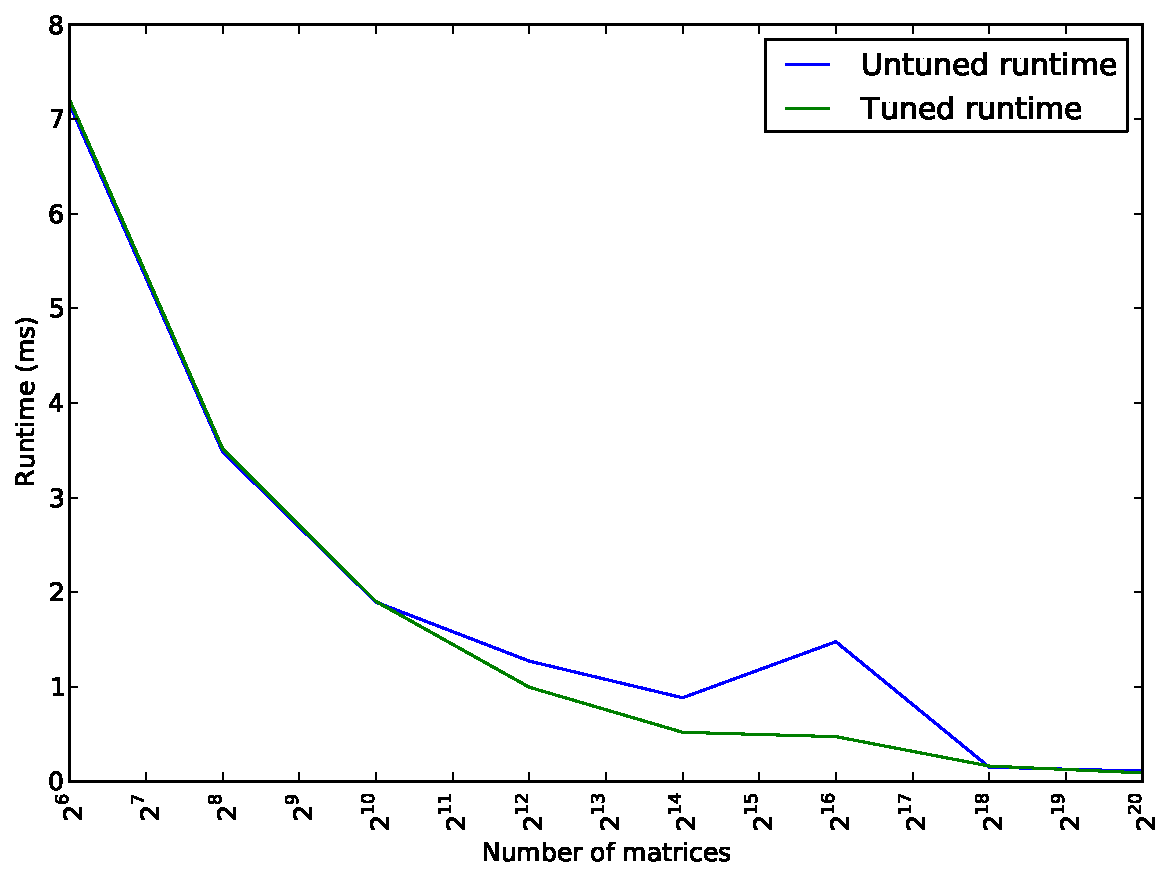
\includegraphics[width=0.8\textwidth]{matrix-inversion}
    \caption{Matrix inversion benchmarks, tuned and untuned.}
    \label{fig:matrix_inv_bench}
\end{figure}

\end{document}
